%!TEX program = xelatex
\documentclass[lang=en,11pt,a4paper,citestyle =authoryear]{elegantpaper}

% 标题
\title{Homework02 - MATH 734}
\author{Boren(Wells) Guan}

% 本文档命令
\usepackage{array,url,stix}
\usepackage{subfigure,listings}
\newcommand{\ccr}[1]{\makecell{{\color{#1}\rule{1cm}{1cm}}}}
\newcommand{\code}[1]{\lstinline{#1}}
\newcommand{\prvd}{$\hfill \qedsymbol$}
\newcommand{\Z}{\mathbb{Z}}
\newcommand{\R}{\mathbb{R}}
\newcommand{\N}{\mathbb{N}}
\newcommand{\C}{\mathbb{C}}
\newcommand{\Q}{\mathbb{Q}}
\newcommand{\M}{\mathcal{M}}
\newcommand{\B}{\mathcal{B}}
\newcommand{\X}{\mathcal{X}}
\newcommand{\Hil}{\mathcal{H}}
\newcommand{\range}{\mathcal{R}}
\newcommand{\nul}{\mathcal{N}}
\newcommand{\F}{\mathcal{F}}

% 文档区
\begin{document}

% 标题
\maketitle

\subsection*{Notation}
Here I use $X \wedge Y$ for $\min(X,Y)$ and $X\vee Y$ for $\max(X,Y)$. r.v. for random variable.

\subsection*{Before Reading:}\par
To make the proof more readable, I will miss or gap some natural or not important facts or notations during my writing. If you feel it hard to see, you can refer the appendix after the proof, where I will try to explain some simple conclusions (will be marked) more clearly. In case that you misunderstand the mark, I will add the mark just after those formulas between \$ and before those between \$\$.\par
And I have to claim that the appendix is of course a part of my assignment, so the reference of it is required. Enjoy your grading!

\subsection*{Ex.1} 
Let $(X_n)_{n\geq 0}$ be a stochastic process defined on a measurable space $(X,\F)$ adpated to a filtration $(\F_n)_{n\geq 0}$. Let $A$ be a measurable subset of the state space. For each $k\geq 1$, let $T_A^{(k)}$ denote the $k^{th}$ time that the process $X_n$ visits some state in $A$. That is
\[
T_A^{(m)} = \begin{cases}\inf\{n>T_A^{(m-1)}, X_n\in A\}\quad&T_A^{(m-1)} < \infty \\ \infty &T_A^{(m-1)} = \infty\end{cases}
\]
Show that $T_A^{(k)}$ is a stopping time for all $k\geq 1$.
\vspace{0.5em}\\
\textbf{Sol.} \par
We know
\[
\{T_A^{(m)} \leq n\} = \bigcup_{k=0}^{\infty}\{\inf\{p>k, X_p \in A\} \leq n, T_A^{(m-1)} = k\} = \bigcup_{k=0}^{n-1} \Big(\bigcup_{i = k+1}^n \{X_i \in A\}\cap\{T_A^{(m-1)} = k\}\Big)
\]
and hence $T_A^{(m-1)}$ is a stopping time will imply that $T_A^{(m)}$ is a stopping time.\par
Then notice
\[
T_A^{(1)} = \inf\{n\geq 0, X_n \in A\}
\]
and hence
\[
\{T_A^{(1)} \leq n\} = \{\inf\{k\geq 0, X_k \in A\} \leq n\} = \bigcup_{k=0}^n\{X_k\in A\} \in \F_n
\]
which means $T_A^{(1)}$ is a stopping time.\par
Therefore, $T_A^{(m)}$ is a stopping time for any $m\geq 1$ by the inducton.
\prvd
\vspace{0.5em}

\subsection*{Ex.2} 
Let $X = (X_n)_{n\geq 0}$ be a supermartingale w.r.t. a filtration $\F_n$ and let $H = (H_n)_{n\geq 1}$ be any predictable sequence w.r.t. $(\F_n)_{n\geq 1}$. Suppose that $H_n$ is bounded and nonnegative for $n\geq 1$. Show that $\int_0^n HdX$ is a supermartingale w.r.t. $\F_n$. Also show the similar results for submartingales and martingales.
\vspace{0.5em}\\
\textbf{Sol.}\par
Notice that $E|\int_0^n HdX| \leq 2M_n\sum\limits_{i=0}^n E|X_i| <\infty$ where $\sup\{|H_i|,1\leq i \leq n\} \leq M_n$,
\[
E(\int_0^{n+1}HdX|\F_n) = E(\sum\limits_{k=1}^{n+1}H_k(X_k-X_{k-1})|\F_n) = H_{n+1}E(X_{n+1}-X_n|\F_n) + \int_0^n HdX \leq \int_0^n HdX
\]
which means $\int_0^n HdX$ is a supermartingale.\par
For submartingales, we claim that $\int_0^n HdX$ is a submartingale w.r.t. $\F_n$ since if $X_n$ is a submartingale, then
\[E(\int_0^{n+1}HdX|\F_n) = E(\sum\limits_{k=1}^{n+1}H_k(X_k-X_{k-1})|\F_n) = H_{n+1}E(X_{n+1}-X_n|\F_n) + \int_0^n HdX \geq \int_0^n HdX\]
and naturally $\int_0^n HdX$ will be a martingale even if $H_n$ may be nonnegative because
\[E(X_{n+1}-X_n|\F_n) = 0\]
for $n\geq 0$ and then we will have
\[
E(\int_0^{n+1}HdX|\F_n) = E(\sum\limits_{k=1}^{n+1}H_k(X_k-X_{k-1})|\F_n) = H_{n+1}E(X_{n+1}-X_n|\F_n) + \int_0^n HdX = \int_0^n HdX
\]
and hence $\int_0^n HdX$ is a martingale.
\prvd
\vspace{0.5em}

\subsection*{Ex.3} 
Find an instance of martingale converging in probability but not almost surely.
\vspace{0.5em}\\
\textbf{Sol.} \par
Let $X_0 = 0$ and $P(X_k = 1|X_{k-1} = 0) = P(X_k = -1|X_{k-1} = 0) = \tfrac{1}{2k}, P(X_k = 0|X_{k-1} = 0) = 1-\tfrac{1}{k}$ and $P(X_k = kX_{k-1}|X_{k-1} \neq 0) = \tfrac{1}{k}, P(X_k = 0|X_{k-1} \neq 0) = 1-\tfrac{1}{k}$, then we know $X_k \to 0$ in probability.\par However, $P(X_k = 0, k\geq K)$ and it picks discrete values and hence $X_k$ can not converge to $0$ a.s. 
\prvd
\vspace{0.5em}

\subsection*{Ex.4} 
Use your favorate programming language (e.g., python, R, matlab, C++) and reproduce plots
similar to the ones in Figure 5.3.1.
\vspace{0.5em}\\
\textbf{Sol.} \par
Here I tried with $(i,j,c) = (1,1,1), (1,1,3), (2,5,7)$ separately and get the images below:
\begin{figure}[htbp]
    \centering
    \subfigure[(1,1,1)]{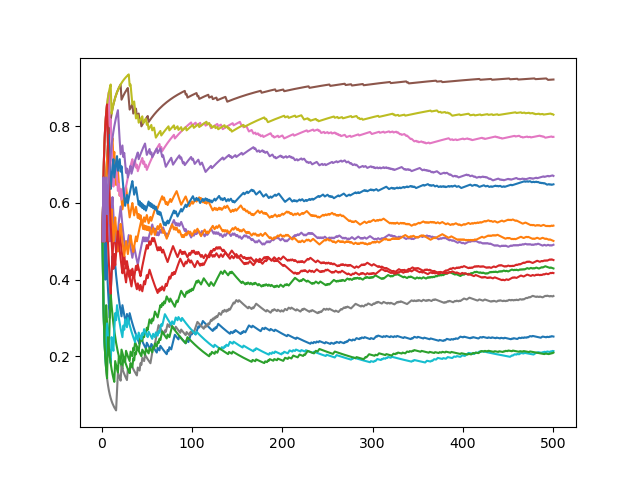
\includegraphics[width = 0.3\textwidth]{Figure_1.png}}
    \subfigure[(1,1,3)]{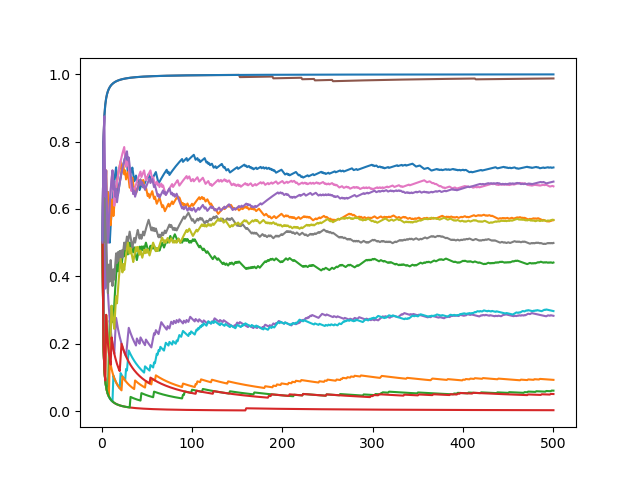
\includegraphics[width = 0.3\textwidth]{Figure_2.png}}
    \subfigure[(2,5,7)]{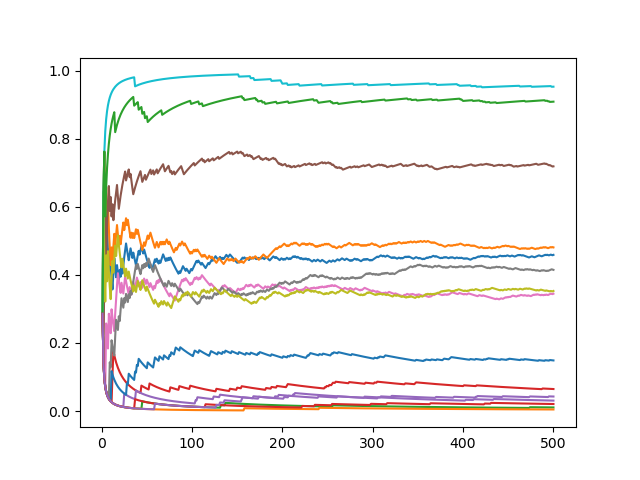
\includegraphics[width = 0.3\textwidth]{Figure_3.png}}
\end{figure}\\
and with the code here:\par
\begin{lstlisting}
import numpy
import matplotlib.pyplot as plt

M = 500
tag = range(1,M+1)
target = []

def simu(i, j, c, target, times = 0, stop = M):
    if times >= stop:
        return
    target.append(i/(i+j))
    t = numpy.random.uniform()
    if t <= i/(i+j):
        simu(i+c,j,c,target,times+1)
    else:
        simu(i,j+c,c,target,times+1)
    return

for i in range(15):
    target = []
    simu(1,1,1,target)
    plt.plot(tag,target)

plt.show()
\end{lstlisting}
\prvd
\vspace{0.5em}

\subsection*{Ex.5} 
Let $X$ be a mean zero r.v. taking values from an interval $[-A,B]$. Fix a convex function $\phi:\R\to\R$. We will show that
\[E(\phi(X)) \leq \phi(-A)\dfrac{B}{A+B} + \phi(B)\dfrac{A}{A+B}\]
In words, over all possible distributions of $X$ over $[-A, B]$, the most extreme distribution that maximizes
$E[\phi(X )]$ is the one that puts point mass on $-A$ and $B$ as in the right-hand side.\par
a. Let $Y$ be a r.v. taking values from $[0, 1]$ and mean $p \in [0, 1]$. Suppose that for any convex function $\phi:\R \to \R$, we have
\[E(\phi(Y)) \leq (1-p)\phi(0) + p\phi(1)\]
then deduce the inequality above.\par
b. Here we will deduce the inequality in (a). Let $Y$ be as before. Let $U \sim \text{Uniform}(0, 1)$ independent from $Y$. Argue that
\[\chi_{U \leq Y }|Y \sim \text{Bernoulli}(Y )\text{ and } \chi_{U \leq Y} \sim \text{Bernoulli}(p)\]
Then use Jensen's inequality to deduce
\[ (1-p)\phi(0)+p\phi(1) = E(\phi(1(U\leq Y))) \geq E(\phi(Y))\]\par
c. Let $\phi(x) = e^{\theta x}$ for a fixed $\theta > 0$ and assume $A = B > 0$. Deduce that
\[E(e^{\theta X}) \leq \dfrac{E(e^{-\theta A})+E(e^{\theta A})}{2} \leq e^{\theta^2 A^2/2}\]
\vspace{0.5em}\\
\textbf{Sol.} \par
a. Let $Y = \dfrac{X}{A+B} + \dfrac{A}{A+B}$ and we know $Y$ is a r.v. taking values from $[0,1]$ and mean $\dfrac{A}{A+B}$, so we know
\[E(f(Y)) \leq \dfrac{B}{A+B}f(0) + \dfrac{A}{A+B} f(1)\]
for any convex function $f:\R\to \R$. Let $f = \phi((A+B)x-A)$ and we will know
\[
\begin{aligned}
f((1-t)x+ty) &= \phi((A+B)[(1-t)x+ty]-A) = \phi((1-t)[(A+B)x-A] + t[(A+B)y-A]) \\ &\leq (1-t)\phi((A+B)x-A)+t\phi((A+B)y-A) = (1-t)f(x) + f(y)
\end{aligned}
\]
for any $x,y\in\R, t\in[0,1]$ and hence $f$ is a convex function, so we will have
\[
E(\phi(X)) = E(f(Y)) \leq \dfrac{B}{A+B}f(0) + \dfrac{A}{A+B} f(1) = \phi(-A)\dfrac{B}{A+B} + \phi(B)\dfrac{A}{A+B}
\]\par
b. Assume $\mu(A) = P(Y\in A)$ and then we know $(U,Y)$ will has the distribution
\[
\int_B du\mu(dy)
\]
and hence $P(\chi_{U\leq Y}|Y \in B) = \int_{(\chi_{U\leq Y} \in B)_Y} du = Y\delta_1(B) + (1-Y)\delta_0(B)$ where
\[
\delta_x(B) = \begin{cases}
    1\quad & x\in B \\
    0&x\notin B
\end{cases}
\]
where $E_Y$ is the $Y$-section, and which means $X_{U\leq Y}|Y \sim \text{Bernoulli}(Y )$. For $\chi_{U\leq Y}$, we know it can be only $1$ or $0$ and where
\[
\begin{aligned}
    P(\chi_{U\leq Y} = 1) &= \int_{U\leq Y} du \mu(dy) = \int \int_{(U\leq Y)_Y} du \mu(dy) = \int Y\mu(dy) = p \\
    P(\chi_{U\leq Y} = 0) &= \int_{(U\leq Y)^c} du \mu(dy) = \int \int_{(U\leq Y)^c_Y} du \mu(dy) = \int (1-Y)\mu(dy) = 1-p
\end{aligned}
\]
then we may know
\[
(1-p)\phi(0)+p\phi(1) = E(\phi(1(U\leq Y)))  = \int \int \phi(\chi(U\leq Y)) du \mu(dy) \geq \int \phi(Y) \mu(dy) = E(\phi(Y))
\]
by the Fubini's theorem and the Jensen's inequality.\par
c. It suffices to show that
\[
\dfrac{E(e^{-\theta A})+E(e^{\theta A})}{2} = \dfrac{e^{-\theta A}+e^{\theta A}}{2} \leq e^{\theta^2A^2/2}
\]
and notice
\[
e^{x^2/2} - (e^x+e^{-x})/2 = \sum\limits_{k=0}^{\infty} (\dfrac{1}{2^kk!}-\dfrac{1}{(2k)!})x^{2k} \geq 0
\]
for any $x\in\R$ since $2^k \leq (2k)!/k!$ for any integer $k$.
\prvd
\vspace{0.5em}

\subsection*{Ex.6} 
Let $T = T (n, p)$ denote the total number of triangles in $G(n, p)$.\par
a. For each three distinct nodes $i , j , k$ in $G$, let $Y_{i,j,k} := \chi_{(i j , jk, ki \in E )}$, which is the indicator variable for the even that there is a triangle with node set ${i , j , k}$. Show that
\[Y_{i,j,k} \sim \text{Bernoulli}(p^3)\]\par
b. Show that we can write
\[T = \sum\limits_{1\leq i < j < k \leq n}\chi_{(i j , jk, ki \in E )}\]\par
Deduce that the expected number of triangles is
\[ET = C_n^3 p^3\]\par
c. Show that
\[\text{var}(T(n,p)) = C_n^3(p^3-p^6) + 12 C_n^4(p^5-p^6) \sim \dfrac{n^4}{2}(p^5-p^6)\]
Thus $\text{Std}(T (n, p)) = \Theta(n^2)$. If CLT holds for $T (n, p)$, then $T (n, p)$ should fluctuate around its mean by $\Theta(n^2)$. Can we
conclude this by CLT?\par
d. Show that for each $t \geq 0$,
\[P\Big(|T(n,p)-C_n^3p^3|\geq t\Big) \leq 2\exp(-\dfrac{t^2}{n(n-1)(n-2)^2})\]
Deduce that the above probability is $o(1)$ if $t\gg n^2$.Specifically, for any $\epsilon > 0$
\[
P\Big(|T(n,p)-C_n^3p^3|\geq n^{2+\epsilon}\Big) \leq 2\exp(-n^{2\epsilon})
\]
Thus, McDirmid's inequality almost confirms the upper tail of fluctuation of $T (n, p)$ predicted by CLT.
\vspace{0.5em}\\
\textbf{Sol.} \par
a. We know
\[
\begin{aligned}
    P(Y_{i,j,k} = 1) &= P(ij,jk,ki\in E) = P(ij\in E)P(jk\in E)P(ki\in E) = p^3 \\
    P(Y_{i,j,k} = 0) &= 1 - P(Y_{i,j,k} = 1) = 1-p^3
\end{aligned}
\]\par
b. We know
\[
T = \sum\limits_{\{i,j,k\}, 1\leq i,j,k\leq n, i\neq j \neq k} Y_{i,j,k} = \sum\limits_{1\leq i < j < k \leq n} Y_{i,j,k} = \sum\limits_{1\leq i < j < k \leq n}\chi_{(i j , jk, ki \in E )}
\]
and hence
\[
ET = E(\sum\limits_{1\leq i < j < k \leq n}\chi_{(i j , jk, ki \in E )}) = E(\sum\limits_{1\leq i < j < k \leq n}Y_{i,j,k}) = \sum\limits_{1\leq i < j < k \leq n}E(Y_{i,j,k}) = C_n^3 p^3
\]\par
c. Denote $N = \{1,2,\cdots, n\}$ and notice
\[\begin{aligned}
ET^2 &= E[(\sum\limits_{1\leq i < j < k \leq n} Y_{i,j,k})^2] = E(\sum\limits_{1\leq i_1 < j_1 < k_1 \leq n}\sum\limits_{1\leq i_2 < j_2 < k_2 \leq n} Y_{i_1,j_1,k_1} Y_{i_2,j_2,k_2}) \\
&= \sum\limits_{1\leq i < j < k \leq n} EY_{i,j,k}^2 + \sum\limits_{1\leq i < j < k\leq n} (\sum\limits_{p\in N-\{i,j,k\}}\sum\limits_{\{m,n\} \subset \{i,j,k\}}EY_{i,j,k}Y_{m,n,p}) \\
&+ \sum\limits_{1\leq i < j < k\leq n} (\sum\limits_{\{p,q\}\subset N-\{i,j,k\}}\sum\limits_{m\in\{i,j,k\}}EY_{i,j,k}Y_{m,p,q}) \\
&+ \sum\limits_{1\leq i < j < k \leq n} \sum\limits_{1\leq p < q < r \leq n, \{i,j,k\}\cap\{p,q,r\} = \emptyset} EY_{i,j,k}Y_{p,q,r} \\
&= C_n^3 p^3 + 3(n-3)C_n^3 p^5 + 3C_n^3C_{n-3}^2p^6 + C_n^3C_{n-3}^3p^6
\end{aligned}
\]
and hence
\[
\begin{aligned}
\text{var}(T(n,p)) = ET^2 -(ET)^2 &= C_n^3 p^3 + 3(n-3)C_n^3 p^5 + 3C_n^3C_{n-3}^2p^6 + C_n^3C_{n-3}^3p^6 - C_n^3C_n^3 p^6 \\
&= C_n^3 p^3 + 12 C_n^4 p^5 + C_n^3(3C_{n-3}^2 + C_{n-3}^3 - C_n^3)p&6 \\
&= C_n^3(p^3-p^6) + 12 C_n^4(p^5-p^6)
\end{aligned}
\]
where you may check that $3C_{n-3}^2 + C_{n-3}^3 - C_n^3 = -3(n-3)-1$. And we have
\[
\lim_{n\to\infty}  \dfrac{C_n^3(p^3-p^6) + 12 C_n^4(p^5-p^6)}{\dfrac{n^4}{2}(p^5-p^6)} = \lim_{n\to\infty} \dfrac{n(n-1)(n-2)(n-3)}{n^4} = 1
\]
and hence 
\[\text{var}(T(n,p)) = C_n^3(p^3-p^6) + 12 C_n^4(p^5-p^6) \sim \dfrac{n^4}{2}(p^5-p^6)\]
By the way, we can not use CLT to $T(n,p)$ since $Y_{i,j,k}$ are not independent at all.\par
d. Let $Y_{i,j}$ be $\chi_{ij\in E}$ and $T$ can be a function as $f(Y_{i,j}):\R^{C_n^2} \to \R$, with $|f(x)-f(x')| \leq n-2$ if $x,x'$ differs on only one corrdinate. So we may use the McDirmid's inequality and we have
\[
P(|T-C_n^3p^3| \geq t) \leq 2\exp\Big(-\dfrac{t^2}{2C_n^2(n-2)^2}\Big) = 2\exp\Big(-\dfrac{t^2}{n(n-1)(n-2)^2}\Big)
\]
then if $t = n^{2+\epsilon}$ for $\epsilon > 0$, we know
\[
P(|T-C_n^3p^3| \geq n^{2+\epsilon}) \leq 2\exp\Big(-n^{2\epsilon}\dfrac{n^{3}}{(n-1)(n-2)^2}\Big) \leq 2\exp(n^{-2\epsilon})
\]
\prvd
\vspace{0.5em}

\subsection*{Durrett 4.3.1.} 
Give an example of a martingale $X_n$ with $\sup_n |X_n| < \infty$ and $P(X_n = a\ i.o.) = 1$ for $a = -1,0,1$. This example shows that it is not enough to have $\sup |X_{n+1} - X_n| < \infty$ in Theorem 4.3.1.
\vspace{0.5em}\\
\textbf{Sol.} \par
Let $\xi_n$ be i.i.d. and $P(\xi_n = 1) = P(\xi_n = -1) = P(\xi_n = 0) = 1/3$ and assume
\[
X_{n+1} = \chi_{X_n = 0}\xi_{n+1} + \chi_{X_n \neq 0}(1+\xi_{n+1})X_n
\]
and $X_0 = \xi_0$. Assume $\F_n = \sigma(\xi_0,\xi_1,\cdots,\xi_n)$ and we may use the induction to show that $X_n \in \F_n$. Notice
\[
E(X_{n+1}|\F_n) = \chi_{X_n\neq 0} X_n = X_n
\]
and we know $X_n$ is a martingale w.r.t. to $\F_n$, also $\sup_n|X_n| < \infty$ but not uniformly bounded. Then we know
\[P(X_n = 0\ i.o.) = 1\] since
\[
P(X_n = 0\ \text{not }i.o.) = \sum\limits_{k\geq 0} P(\bigcap_{m\geq k}\{X_m \neq 0\}) = 0
\]
and hence $P(X_n = 1\ i.o.) = P(X_n = -1\ i.o.) = 1$.
\prvd
\vspace{0.5em}

\subsection*{Durrett 4.3.2.} 
(Assumes familiarity with finite state Markov chains.) Fine tune the example for the previous problem so that $P (X_n = 0) \to 1 - 2p$ and $P(X_n = -1), P(X_n = 1) \to p$, where $p$ is your favorite number in $(0,1/2$), i.e., you are asked to do this for one value of $p$ that you may choose. This example shows that a martingale can converge in distribution without converging a.s. (or in probability).
\vspace{0.5em}\\
\textbf{Sol.} \par
Assume $\xi_n$ independent with
\[
P(\xi_k = k-i) = \dfrac{1}{4k}+\dfrac{1}{2k^2},\quad P(\xi_k = -(k-i)) =  \dfrac{1}{4k}+\dfrac{1}{2k^2},\quad P(\xi_k = 0) = \dfrac{1}{2} - \dfrac{1}{k}, 
\]
for $1\leq i \leq k$ and let $\F_n = \sigma(\xi_1,\cdots,Y\xi_n)$ and we know
\[
X_{n+1} = \xi_{n+1}\chi_{X_n = 0} + \dfrac{4n}{(n+2)(n-1)}X_n|\xi_{n+1}|\chi_{X_{n}\neq 0}
\]
and we know $X_n \in \F_n$ by the induction, then
\[
E(X_{n+1}|\F_n) = \chi_{X_n\neq 0}X_n = X_n
\]
Then \[P(X_{n+1} = 0) = (\dfrac{1}{2}-\dfrac{1}{n+1})P(X_n = 0) + (\dfrac{1}{2}-\dfrac{1}{n+1})(1-P(X_n = 0)) = \dfrac{1}{2}-\dfrac{1}{n+1} \to \dfrac{1}{2}\] and
\[
P(X_{n+1} = 1) = (\dfrac{1}{2}-\dfrac{1}{n})(\dfrac{1}{2} - \dfrac{1}{n})+(\dfrac{1}{2}+\dfrac{1}{n})P(X_n = \dfrac{1}{2}+\dfrac{1}{n+1}) = \dfrac{1}{4}- \dfrac{1}{4(n+1)^2} \to \dfrac{1}{4}
\]
and $P(X_{n+1} = -1)$ is similar.

\prvd
\vspace{0.5em}

\subsection*{Durrett Ex.4.3.3} 
Let $X_n$ and $Y_n$ be positive integrable and adapted to $\F_n$. Suppose $E(X_{n+1}|\F_n) \leq X_n + Y_n$, with $\sum Y_n < \infty$ a.s. Prove that $X_n$ converges a.s. to a finite limit.
\vspace{0.5em}\\
\textbf{Sol.} \par
Let $S_n = X_n - \sum\limits_{k=1}^{n-1}Y_k$ and we know
\[
E(S_{n+1}|\F_n) = E(X_{n+1}|\F_n) - Y_n - (X_n - S_n) \leq X_n - (X_n - S_n) = S_n
\]
which means $S_n$ is a supermartingale. Assume $M>0$ and
\[N = \inf\{k,\sum\limits_{i=1}^k Y_k > M\}\]
then we know
\[S_{n\wedge N} + M \geq X_{n\wedge N} \geq 0\]
and hence $S_{n\wedge N} + M$ will converge to a finite limit almost surely since $S_{n\wedge N}$ is also a supermartingale.\par
Now it is suffice to show that $S_n$ converges to a finite limit a.s. since $X_n = S_n + \sum\limits_{i=1}^{n-1}Y_i$ where $\sum\limits_{i=1}^{n-1}Y_i$ converges to $\sum\limits_{i=1}^{\infty} Y_i < \infty$ a.s. For all $\omega \in \{\omega,\sum\limits_{i=1}^{\infty} Y_i(\omega)< M\}$, we know $N(M) = \infty$ and hence $S_{n\wedge N}(\omega) = S_n(\omega)$, then we know $S_n(\omega)$ converges to a finite limit a.s. on $\{\omega,\sum\limits_{i=1}^{\infty} Y_i(\omega)<M\}$, and hence $S_n$ will converge to a finite limit a.s. on $\bigcup_{M=0}^{\infty}\{\omega,\sum\limits_{i=1}^{\infty} Y_i(\omega)<M\}$ and notice
\[\bigcup_{M=0}^{\infty}\{\omega,\sum\limits_{i=1}^{\infty} Y_i(\omega)<M\} = \Omega\]
and hence $S_n$ converges to a finite limit a.s. 
\prvd
\vspace{0.5em}

\subsection*{Durrett Ex.4.3.4.} 
Let $p_m \in [0, 1)$. Use the Borel-Cantelli lemmas to show that
\[
\prod_{m=1}^{\infty}(1-p_m) = 0\iff \sum\limits_{m=1}^{\infty}p_m = \infty
\]
\vspace{0.5em}\\
\textbf{Sol.} \par
Let $B_n$ be independent events with $P(B_n) = p_n$ and $\F_n = \sigma(\{\emptyset, \Omega,B_1,\cdots,B_n \})$ and $\F_0 = \{\emptyset,\Omega\}$. By the Second Borel-Cantelli's Lemma, we know
\[
1 - \prod_{m=1}^{\infty}(1-p_m) \geq P(B_n\ i.o.) = P(\sum\limits_{n=1}^{\infty} P(B_n|\F_{n-1}) = \infty) = P(\sum\limits_{n=1}^{\infty} p_n = \infty)
\]
and
\[
1 - \sum\limits_{k\geq 1}\prod_{m=k}^{\infty}(1-p_m) \leq P(B_n\ i.o.) = P(\sum\limits_{n=1}^{\infty} p_n = \infty)
\]
since $B_n$ is independent to $\F_{n-1}$ and hence if $\sum\limits_{m=1}^{\infty} p_m = \infty$, we know
\[
\prod_{m=1}^{\infty}(1-p_m) \leq 1 - P(\sum\limits_{n=1}^{\infty} \chi_{B_n} = \infty) = 0
\]
which means $\prod_{m=1}^{\infty}(1-p_m) = 0$. If $\prod_{m=1}^{\infty}(1-p_m) = 0$, then we know $\prod_{m=k}^{\infty}(1-p_m) = 0$ for any integer $k$ and hence
\[1 = 1 - \sum\limits_{k\geq 1}\prod_{m=k}^{\infty}(1-p_m) \leq  P(\sum\limits_{n=1}^{\infty} p_n = \infty)\]
which means $\sum\limits_{n=1}^{\infty} p_n = \infty$ since $P(\sum\limits_{n=1}^{\infty} p_n = \infty)$ can be only $0$ or $1$.

\prvd
\vspace{0.5em}

\addappheadtotoc

\end{document}
